\section{Benchmarking scaled matrix multiplication implementation in PyTorch} 
\label{app:scaled_mm_benchmarking}

\begin{figure}[!h]
    % \vspace{4em}
    \centering
    \begin{subfigure}{\textwidth}
        \centering
        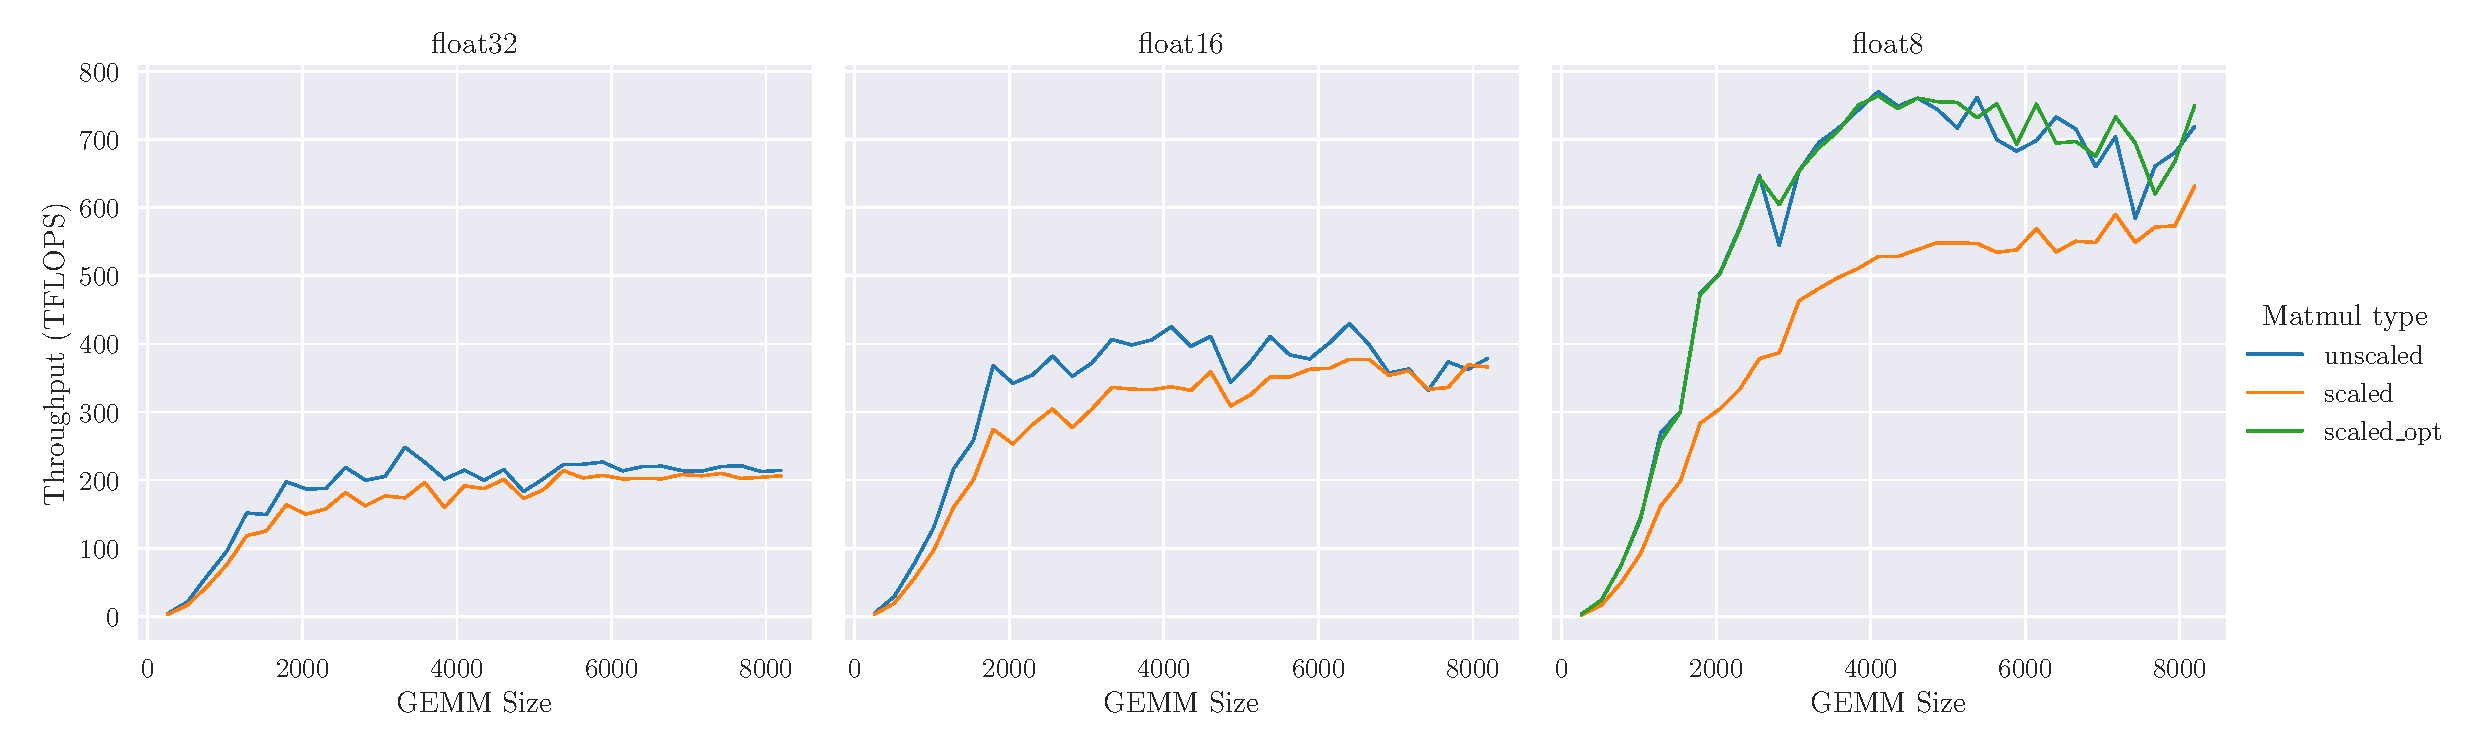
\includegraphics[width=\textwidth]{arXiv/figures/scaled-mm-benchmarking.pdf}
    \end{subfigure}
    \caption{Square matrix multiplication throughput in TFLOPs with and without scaling factors applied to the output across 32-, 16-, and 8-bit float dtypes on NVIDIA H100 PCIe. Naive implementation in PyTorch.}
    \label{fig:scaled-mm-benchmarking}
\end{figure}

Standard strategies for FP8 training require expensive statistics gathering (e.g., amax) per tensor. A key benefit of \umup\ for FP8 training is that it instead provides us with static scaling factors to rescale operation outputs. Even a naive implementation in pytorch can achieve a minimal drop in hardware utilization.

Figure \ref{fig:scaled-mm-benchmarking} demonstrates hardware utilization for FP8, FP16, and FP32 matrix multiplications on a single NVIDIA H100 PCIe card. For FP16 and FP32, \texttt{torch.matmul} is used, whereas \texttt{torch.\_scaled\_mm} is used for FP8. Comparing "scaled" to "unscaled" matrix multiplication demonstrates a 30$\%$, 20$\%$, and 10$\%$ drop in hardware utilization for each data type respectively. In the case of FP8, where the drop in utilization is most pronounced, utilization can be recovered by passing the scaling factor as a scale associated with one of the two input tensors.

It should be noted that as of PyTorch version 2.3, \texttt{torch.\_scaled\_mm} always computes amax as well as the matrix multiplication. The performance of FP8 matrix multiplications could be higher without this overhead.